\documentclass[12pt,a4paper]{article}
% 基础包
\usepackage{ctex}
\usepackage{geometry}
\usepackage{fancyhdr}
\usepackage{lastpage}
\usepackage{indentfirst}
% 字体设置
\usepackage{mathptmx}
\usepackage[T1]{fontenc}
% 数学公式
\usepackage{amsmath,amssymb,amsfonts}
\usepackage{mathtools}
\usepackage{nccmath}
\everymath{\displaystyle}
\usepackage{txfonts}
\providecommand{\varparallel}{\mathrel{/\!/}}
% 表格
\usepackage{array}
\usepackage{booktabs}
\usepackage{multirow}
\usepackage{colortbl}
% 图片和颜色
\usepackage{graphicx}
\usepackage{xcolor}
\usepackage{caption}
\usepackage{subcaption}
% 列表
\usepackage{enumitem}
\usepackage{tasks}
% TikZ 画图
\usepackage{tikz}
\usepackage{tikz-3dplot}
\usetikzlibrary{
	arrows.meta, calc, patterns, intersections,
	through, angles, quotes, decorations.pathmorphing
}
% 页面设置
\geometry{
	left=1.6cm,
	right=2.04cm,
	top=1.6cm,
	bottom=2.54cm,
	headheight=1.2cm,
	footskip=0.8cm,
	nohead
}
% 行距和段落
\linespread{1.5}
\setlength{\parindent}{2em}
\setlength{\parskip}{0.5ex}
% 页脚设置
\pagestyle{fancy}
\fancyhf{}
\fancyfoot[C]{\makebox[0pt][c]{数学试题~第\thepage 页（共\pageref{LastPage}页）}}
\renewcommand{\headrulewidth}{0pt}
\renewcommand{\footrulewidth}{0pt}
% 选择题选项环境
\NewTasksEnvironment[
label=\Alph*.,
label-width=1.5em,
item-indent=2em,
column-sep=2em,
before-skip=0.8em,
after-skip=0.8em
]{choicesFour}[\choice](4)
\NewTasksEnvironment[
label=\Alph*.,
label-width=1.5em,
item-indent=2em,
column-sep=3em,
before-skip=0.8em,
after-skip=0.8em
]{choicesTwo}[\choice](2)
\NewTasksEnvironment[
label=\Alph*.,
label-width=1.5em,
item-indent=2em,
before-skip=0.8em,
after-skip=0.8em
]{choicesOne}[\choice](1)
\begin{document}
	\noindent {\large\bfseries 绝密$\bigstar$启用前}
	
	\vspace*{0.5cm}
	
	% 封面部分
	\begin{center}
		{\Large 2025年普通高等学校招生全国统一考试}\\[0.8cm]
		{\LARGE\bfseries 数~~~~学（答案解析版）}
	\end{center}
	
	\vspace{0.3cm}
	
	\noindent\hangindent=2em {\bfseries 一、选择题：本题共8小题，每小题5分，共40分. 每小题给出的四个选项中，只有一项是符合题目要求的.}
	\begin{enumerate}[leftmargin=*,label=\arabic*.,itemsep=0.8ex]
		\item $(1+5\mathrm{i})\mathrm{i}$的虚部为
		\begin{choicesFour}
			\choice $-1$ \choice $0$ \choice $1$ \choice $6$
		\end{choicesFour}
		\textbf{【答案】C}
		
		\textbf{【详解】}因为$(1+5\mathrm{i})\mathrm{i}=\mathrm{i}+5\mathrm{i}^2=-5+\mathrm{i}$，
		
		所以其虚部为$1$，
		
		故选C.
		
		\item 设全集$U=\{x\mid x\text{是小于}9\text{的正整数}\}$，集合$A=\{1,3,5\}$，则$\complement_U A$中元素个数为
		\begin{choicesFour}
			\choice $0$ \choice $3$ \choice $5$ \choice $8$
		\end{choicesFour}
		\textbf{【答案】C}
		
		\textbf{【详解】}因为$U=\{1,2,3,4,5,6,7,8\}$，
		
		所以$\complement_U A=\{2,4,6,7,8\}$，
		
		所以$\complement_U A$中的元素个数为$5$，
		
		故选C.
		
		\item 若双曲线$C$的虚轴长为实轴长的$\sqrt7$倍，则$C$的离心率为
		\begin{choicesFour}
			\choice $\sqrt2$ \choice $2$ \choice $\sqrt7$ \choice $2\sqrt2$
		\end{choicesFour}
		\textbf{【答案】D}
		
		\textbf{【详解】}设双曲线的实轴、虚轴、焦距分别为$2a,2b,2c$.
		
		由题知$b=\sqrt7 a$，
		
		于是$c=\sqrt{a^2+b^2}=2\sqrt2 a$，
		
		则$e=\dfrac{c}{a}=2\sqrt2$，
		
		故选D.
		
		\item 若点$(a,0)\ (a>0)$是函数$y=2\tan\left(x-\dfrac{\pi}{3}\right)$的图象的一个对称中心，则$a$的最小值为
		\begin{choicesFour}
			\choice $\dfrac{\pi}{6}$ \choice $\dfrac{\pi}{3}$ \choice $\dfrac{\pi}{2}$ \choice $\dfrac{4\pi}{3}$
		\end{choicesFour}
		\textbf{【答案】B}
		
		\textbf{【详解】}根据正切函数的性质，$y=2\tan\left(x-\dfrac{\pi}{3}\right)$的对称中心横坐标满足$x-\dfrac{\pi}{3}=\dfrac{k\pi}{2}\ (k\in\mathbb{Z})$，
		
		即$x=\dfrac{\pi}{3}+\dfrac{k\pi}{2}$.
		
		又$a>0$，
		
		则$k=0$时$a$最小，最小值是$\dfrac{\pi}{3}$，
		
		故选B.
		
		\item 设$f(x)$是定义在$\mathbb{R}$上且周期为$2$的偶函数，当$2\le x\le3$时，$f(x)=5-2x$，则$f\left(-\dfrac34\right)=$
		\begin{choicesFour}
			\choice $-\dfrac12$ \choice $-\dfrac14$ \choice $\dfrac14$ \choice $\dfrac12$
		\end{choicesFour}
		\textbf{【答案】A}
		
		\textbf{【详解】}由题知$f(x+2)=f(x)$，$f(-x)=f(x)$对一切$x$成立，
		
		于是$f\left(-\dfrac34\right)=f\left(\dfrac34\right)=f\left(\dfrac34+2\right)=f\left(\dfrac{11}{4}\right)=5-2\times\dfrac{11}{4}=-\dfrac12$，
		
		故选A.
		
		\item 帆船比赛中，运动员可借助风力计测定风速的大小和方向，测出的结果在航海学中称为视风风速，视风风速对应的向量，是真风风速对应的向量与船行风速对应的向量之和，其中船行风速对应的向量与船速对应的向量大小相等，方向相反. 图1给出了部分风力等级、名称与风速大小的对应关系. 已知某帆船运动员在某时刻测得的视风风速对应的向量与船速对应的向量如图2（风速的大小和向量的大小相同），单位（m/s），则真风为
		
		\noindent\begin{minipage}[t]{0.4\linewidth}
			\vspace*{0pt}% 统一顶部基线，使两个minipage顶端对齐
			\centering
			\begin{tabular}{|c|c|c|}
				\hline
				等级 & 风速大小(m/s) & 名称 \\
				\hline
				$2$ & $1.1\sim3.3$ & 轻风 \\
				\hline
				$3$ & $3.4\sim5.4$ & 微风 \\
				\hline
				$4$ & $5.5\sim7.9$ & 和风 \\
				\hline
				$5$ & $8.0\sim10.1$ & 劲风 \\
				\hline
			\end{tabular}\\[0.3em]
			图1
		\end{minipage}\hfill
		\begin{minipage}[t]{0.6\linewidth}
			\vspace*{0pt}% 统一顶部基线，使两个minipage顶端对齐
			\centering
			\begin{tikzpicture}[baseline=(current bounding box.north), scale=1, line cap=round, line join=round, >=Stealth]
				\draw[gray!30, step=1, dashed] (0,0) grid (3,3);
				\draw[->] (0,0)--(3.5,0);
				\draw[->] (0,0)--(0,3.5);
				\draw[->, thick] (3,3)--(0,2) node[above left]{视风};
				\draw[->, thick] (2,0)--(3,3) node[above right]{船速};
				\fill (0,0) circle(2pt) node[below left]{$O$};
			\end{tikzpicture}\\[0.3em]
			图2
		\end{minipage}
		\begin{choicesFour}
			\choice 轻风 \choice 微风 \choice 和风 \choice 劲风
		\end{choicesFour}
		\textbf{【答案】A}
		
		\textbf{【详解】}由题意及图2得，视风风速对应的向量为$(-3,-1)$，船速对应的向量为$(1,3)$，
		
		故船行风速对应的向量为$(-1,-3)$.
		
		设真风风速对应的向量为$\boldsymbol{v}$，
		
		则$(-3,-1)=\boldsymbol{v}+(-1,-3)$，
		
		所以$\boldsymbol{v}=(-3,-1)-(-1,-3)=(-2,2)$，
		
		$|\boldsymbol{v}|=2\sqrt2\approx2.8$.
		
		由表得，真风风速为轻风，
		
		故选A.
		
		\item 若圆$x^2+(y+2)^2=r^2\ (r>0)$上到直线$y=\sqrt3x+2$的距离为$1$的点有且仅有$2$个，则$r$的取值范围是
		\begin{choicesFour}
			\choice $(0,1)$ \choice $(1,3)$ \choice $(3,+\infty)$ \choice $(0,+\infty)$
		\end{choicesFour}
		\textbf{【答案】B}
		
		\textbf{【详解】}圆心$(0,-2)$到直线$\sqrt3x-y+2=0$的距离为$d=\dfrac{|2+2|}{2}=2$.
		
		到直线距离为$1$的点在与该直线平行、距离为$1$的两条直线$y=\sqrt3x$与$y=\sqrt3x+4$上，
		
		它们到圆心的距离分别为$1$和$3$.
		
		当$r=1$时圆上只有$1$个点到直线距离为$1$；
		
		当$r=3$时圆上有$3$个；
		
		故有且仅有$2$个点时，$1<r<3$，
		
		故选B.
		
		\begin{center}
			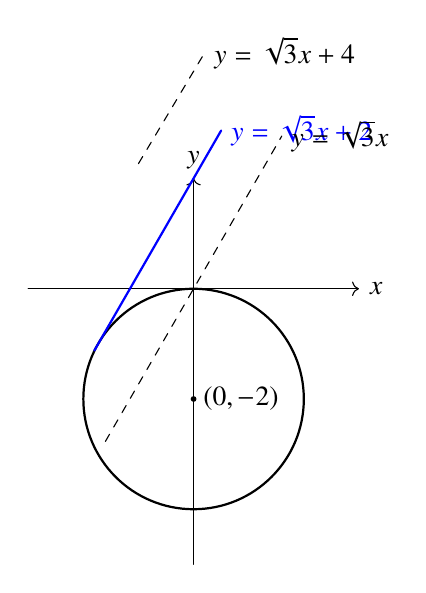
\begin{tikzpicture}[scale=0.7, line cap=round, line join=round]
				\draw[->] (-3,0)--(3,0) node[right]{$x$};
				\draw[->] (0,-5)--(0,2) node[above]{$y$};
				\draw[thick] (0,-2) circle (2);
				\draw[thick, blue] (-1.8,-1.12)--(0.5,2.87) node[right]{$y=\sqrt3x+2$};
				\draw[dashed] (-1.6,-2.77)--(1.6,2.77) node[right]{$y=\sqrt3x$};
				\draw[dashed] (-1,2.27)--(0.2,4.28) node[right]{$y=\sqrt3x+4$};
				\fill (0,-2) circle(1.5pt) node[right]{$(0,-2)$};
			\end{tikzpicture}
		\end{center}
		
		\item 若实数$x,y,z$满足$2+\log_2 x=3+\log_3 y=5+\log_5 z$，则$x,y,z$的大小关系不可能是
		\begin{choicesFour}
			\choice $x>y>z$ \choice $x>z>y$ \choice $y>x>z$ \choice $y>z>x$
		\end{choicesFour}
		\textbf{【答案】B}
		
		\textbf{【详解】}设$2+\log_2 x=3+\log_3 y=5+\log_5 z=t$，
		
		则$x=2^{t-2}$，$y=3^{t-3}$，$z=5^{t-5}$.
		
		令$t=4$，则$x=4,\ y=3,\ z=0.2$，此时$x>y>z$，A有可能；
		
		令$t=5$，则$x=8,\ y=9,\ z=1$，此时$y>x>z$，C有可能；
		
		令$t=8$，则$x=64,\ y=243,\ z=125$，此时$y>z>x$，D有可能；
		
		故选B.
		
	\end{enumerate}
	\vspace{0.3cm}
	\noindent\hangindent=2em {\bfseries 二、选择题：本题共3小题，每小题6分，共18分. 每小题给出的选项中，有多项符合题目要求. 全部选对的得6分，部分选对的得部分分，有选错的得0分.}
	\begin{enumerate}[leftmargin=*,label=\arabic*.,resume,itemsep=0.8ex]
		\item 在正三棱柱$ABC-A_1B_1C_1$中，$D$为$BC$中点，则
		\begin{choicesFour}
			\choice $AD\perp A_1C$ \choice $BC\perp$平面$AA_1D$ \choice $AD\varparallel A_1B_1$ \choice $CC_1\varparallel$平面$AA_1D$
		\end{choicesFour}
		\textbf{【答案】BD}
		
		\textbf{【详解】}设底边为$a$.
		
		对于A：$\overrightarrow{AD}\cdot\overrightarrow{A_1C}=\dfrac12(\overrightarrow{AB}+\overrightarrow{AC})\cdot(\overrightarrow{AC}-\overrightarrow{AA_1})=\dfrac12\left(\dfrac{a^2}{2}+a^2-0-0\right)=\dfrac{3a^2}{4}\ne0$，
		
		故$AD\perp A_1C$不成立，A错误；
		
		对于B：正三棱柱中$AA_1\perp$平面$ABC$，则$AA_1\perp BC$，
		
		又$\triangle ABC$为正三角形，$D$为$BC$中点，则$AD\perp BC$，
		
		$AA_1\cap AD=A$，
		
		所以$BC\perp$平面$AA_1D$，B正确；
		
		对于C：若$AD\varparallel A_1B_1$，则$AD\varparallel AB$，矛盾，C错误；
		
		对于D：$CC_1\varparallel AA_1$，$AA_1\subset$平面$AA_1D$，$CC_1\not\subset$平面$AA_1D$，
		
		所以$CC_1\varparallel$平面$AA_1D$，D正确.
		
		故选BD.
		
		\item 设抛物线$C:y^2=6x$的焦点为$F$，过$F$的直线交$C$于$A,B$，过$F$且垂直于$AB$的直线交$l:x=-\dfrac32$于$E$，过点$A$作准线$l$的垂线，垂足为$D$，则
		\begin{choicesTwo}
			\choice $|AD|=|AF|$
			\choice $|AE|=|AB|$
			\choice $|AB|\ge6$
			\choice $|AE|\cdot|BE|\ge18$
		\end{choicesTwo}
		\textbf{【答案】ACD}
		
		\textbf{【详解】}对于A：$l$为准线，由抛物线定义知$|AD|=|AF|$，A正确；
		
		对于B：取通径情形，$A\left(\dfrac32,3\right),B\left(\dfrac32,-3\right),E\left(-\dfrac32,0\right)$，
		
		则$|AE|=3\sqrt2\ne6=|AB|$，B错误；
		
		对于C：设直线$AB:x=my+\dfrac32$，联立$y^2=6x$得$y^2-6my-9=0$，
		
		则$x_1+x_2=m(y_1+y_2)+3=6m^2+3$，
		
		$|AB|=x_1+x_2+3=6m^2+6\ge6$，当$m=0$时取等号，C正确；
		
		对于D：因$EF\perp AB$，$|AE|^2=|AF|^2+|EF|^2$，$|BE|^2=|BF|^2+|EF|^2$，
		
		结合焦半径公式计算可得$|AE|\cdot|BE|\ge18$，当且仅当$m=0$时取等号，D正确.
		
		故选ACD.
		
		\item 已知$\triangle ABC$的面积为$\dfrac14$，若$\cos2A+\cos2B+2\sin^2C=2$，$\cos A\cos B\sin C=\dfrac14$，则
		\begin{choicesTwo}
			\choice $\sin C=\sin^2A+\sin^2B$
			\choice $AB=\sqrt2$
			\choice $\sin A+\sin B=\dfrac{\sqrt6}{2}$
			\choice $AC^2+BC^2=3$
		\end{choicesTwo}
		\textbf{【答案】ABC}
		
		\textbf{【详解】}由二倍角公式，$1-2\sin^2A+1-2\sin^2B+2\sin^2C=2$，
		
		整理得$\sin^2C=\sin^2A+\sin^2B$，
		
		由正弦定理得$c^2=a^2+b^2$，
		
		所以$C=\dfrac{\pi}{2}$，$\sin C=1$，
		
		则$\sin C=\sin^2A+\sin^2B$，A正确；
		
		由$\cos A\cos B\sin C=\dfrac14$得$\cos A\sin A=\dfrac14$，即$\sin2A=\dfrac12$，
		
		由面积$\dfrac12 ab\sin C=\dfrac14$得$ab=\dfrac12$，
		
		又$a=c\sin A$，$b=c\cos A$，
		
		所以$ab=c^2\sin A\cos A=\dfrac{c^2}{4}=\dfrac12$，
		
		解得$c^2=2$，$AB=c=\sqrt2$，B正确；
		
		$(\sin A+\sin B)^2=(\sin A+\cos A)^2=1+\sin2A=\dfrac32$，
		
		所以$\sin A+\sin B=\dfrac{\sqrt6}{2}$，C正确；
		
		$AC^2+BC^2=AB^2=2\ne3$，D错误.
		
		故选ABC.
		
	\end{enumerate}
	\vspace{0.3cm}
	\noindent {\bfseries 三、填空题：本题共3小题，每小题5分，共15分.}
	\begin{enumerate}[leftmargin=*,label=\arabic*.,resume,itemsep=0.8ex]
		\item 若直线$y=2x+5$是曲线$y=\mathrm{e}^x+x+a$的切线，则$a=$\underline{\quad$4$\quad}.
		
		\textbf{【详解】}对$y=\mathrm{e}^x+x+a$，其导数为$y'=\mathrm{e}^x+1$.
		
		令$\mathrm{e}^x+1=2$，解得$x=0$.
		
		将$x=0$代入切线方程$y=2x+5$，可得$y=5$，
		
		所以切点坐标为$(0,5)$.
		
		因为切点在曲线上，
		
		所以$\mathrm{e}^0+0+a=5$，即$1+a=5$，
		
		解得$a=4$.
		
		\item 若一个等比数列的各项均为正数，且前$4$项和为$4$，前$8$项和为$68$，则该等比数列的公比为\underline{\quad$2$\quad}.
		
		\textbf{【详解】}设公比为$q$，
		
		则$S_4=\dfrac{a_1(1-q^4)}{1-q}=4$，$S_8=\dfrac{a_1(1-q^8)}{1-q}=68$.
		
		两式相除得$1+q^4=17$，即$q^4=16$，
		
		所以$q=2$（各项均为正数，舍去负值）.
		
		\item 一个箱子里有$5$个相同的球，分别以$1\sim5$标号，若每次取一颗，有放回地取三次，记至少取出一次的球的个数$X$，则数学期望$E(X)=$\underline{\quad$\dfrac{61}{25}$\quad}.
		
		\textbf{【详解】}记$X_i$表示第$i$号球至少被取出一次，
		
		则$P(X_i=1)=1-\left(\dfrac45\right)^3=\dfrac{61}{125}$.
		
		由期望的线性性质，
		
		$E(X)=\sum\limits_{i=1}^5 E(X_i)=5\times\dfrac{61}{125}=\dfrac{61}{25}$.
		
	\end{enumerate}
	\vspace{0.3cm}
	\noindent {\bfseries 四、解答题：本题共5小题，共77分. 解答应写出文字说明、证明过程或演算步骤.}
	\begin{enumerate}[leftmargin=*,label=\arabic*.,resume,itemsep=1.2ex]
		\item (13分)\\
		为研究某疾病与超声波检查结果的关系，从做过超声波检查的人群中随机调查了$1000$人，得到如下列联表：
		\begin{center}
			\begin{tabular}{|c|c|c|c|}
				\hline
				超声波检查结果 组别 & 正常 & 不正常 & 合计 \\
				\hline
				患该疾病 & $20$ & $180$ & $200$ \\
				\hline
				未患该疾病 & $780$ & $20$ & $800$ \\
				\hline
				合计 & $800$ & $200$ & $1000$ \\
				\hline
			\end{tabular}
		\end{center}
		(1) 记超声波检查结果不正常者患该疾病的概率为$P$，求$P$的估计值；
		
		(2) 根据小概率值$\alpha=0.001$的独立性检验，分析超声波检查结果是否与患该疾病有关.
		
		附：$\chi^2=\dfrac{n(ad-bc)^2}{(a+b)(c+d)(a+c)(b+d)}$，
		\begin{center}
			\begin{tabular}{|c|c|c|c|}
				\hline
				$P(\chi^2\ge k)$ & $0.005$ & $0.010$ & $0.001$ \\
				\hline
				$k$ & $3.841$ & $6.635$ & $10.828$ \\
				\hline
			\end{tabular}
		\end{center}
		\textbf{【答案】}(1) $0.9$；(2) 有关.
		
		\textbf{【详解】}(1) 根据表格可知，检查结果不正常的$200$人中有$180$人患病，
		
		所以$P$的估计值为$\dfrac{180}{200}=0.9$.
		
		(2) 零假设为$H_0$：超声波检查结果与患病无关.
		
		根据表中数据可得
		\[
		\chi^2=\frac{1000\times(20\times20-180\times780)^2}{200\times800\times800\times200}=765.625>10.828.
		\]
		
		根据小概率值$\alpha=0.001$的独立性检验，我们推断$H_0$不成立，
		
		即认为超声波检查结果与患该病有关，该推断犯错误的概率不超过$0.001$.
		
		\item (15分)\\
		设数列$\{a_n\}$满足$a_1=3$，$\dfrac{a_{n+1}}{n}=\dfrac{a_n}{n+1}+\dfrac{1}{n(n+1)}$.
		
		(1) 证明：$\{na_n\}$为等差数列；
		
		(2) 设$f(x)=a_1x+a_2x^2+\cdots+a_mx^m$，求$f'(-2)$.
		
		\textbf{【答案】}(2) $f'(-2)=\dfrac{7-(3m+7)(-2)^m}{9}$.
		
		\textbf{【详解】}(1) 在数列$\{a_n\}$中，$\dfrac{a_{n+1}}{n}=\dfrac{a_n}{n+1}+\dfrac{1}{n(n+1)}$，
		
		两边同乘$n(n+1)$，得$(n+1)a_{n+1}=na_n+1$，
		
		即$(n+1)a_{n+1}-na_n=1$，
		
		所以$\{na_n\}$是以$1\times a_1=3$为首项、$1$为公差的等差数列.
		
		(2) 由(1)得$na_n=3+(n-1)=n+2$，即$a_n=\dfrac{n+2}{n}$.
		
		于是
		\[
		f'(x)=\sum_{n=1}^m na_nx^{n-1}=\sum_{n=1}^m (n+2)x^{n-1},
		\]
		\[
		f'(-2)=\sum_{n=1}^m (n+2)(-2)^{n-1}.
		\]
		
		用错位相减：设$S=\sum\limits_{n=1}^m (n+2)(-2)^{n-1}$，
		
		则$-2S=\sum\limits_{n=1}^m (n+2)(-2)^{n}$，
		
		两式相减得
		\[
		3S=3+\sum_{n=1}^{m-1}(-2)^n-(m+2)(-2)^m,
		\]
		
		整理得
		\[
		f'(-2)=S=\frac{7-(3m+7)(-2)^m}{9}.
		\]
		
		\item (15分)\\
		如图所示的四棱锥$P-ABCD$中，$PA\perp$平面$ABCD$，$BC\varparallel AD$，$AB\perp AD$.
		
		(1) 证明：平面$PAB\perp$平面$PAD$；
		
		(2) $PA=AB=\sqrt2$，$AD=1+\sqrt3$，$BC=2$，$P,B,C,D$在同一个球面上，设该球面的球心为$O$.
		
		\hspace*{2em}(i) 证明：$O$在平面$ABCD$上；
		
		\hspace*{2em}(ii) 求直线$AC$与直线$PO$所成角的余弦值.
		
		\begin{flushright}
			\tdplotsetmaincoords{70}{200}
			\begin{tikzpicture}[tdplot_main_coords, baseline=(current bounding box.north), scale=2, line cap=round, line join=round]
				\coordinate (D) at (0,0,0);
				\coordinate (A) at (2.73,0,0);
				\coordinate (B) at (2.73,1.41,0);
				\coordinate (C) at (0.73,1.41,0);
				\coordinate (P) at (2.73,0,1.41);
				\draw[thick] (P)--(B) (C)--(B) (D)--(C) (C)--(P) (D)--(P);
				\draw[dashed] (A)--(D) (A)--(B) (P)--(A);
				\fill (A) circle(1pt) node[below left]{$A$};
				\fill (B) circle(1pt) node[below right]{$B$};
				\fill (C) circle(1pt) node[right]{$C$};
				\fill (D) circle(1pt) node[above left]{$D$};
				\fill (P) circle(1pt) node[above]{$P$};
			\end{tikzpicture}
		\end{flushright}
		\textbf{【答案】}(2)(ii) $\dfrac{\sqrt2}{3}$.
		
		\textbf{【详解】}(1) 在四棱锥中，$PA\perp$平面$ABCD$，$AB\subset$平面$ABCD$，$AD\subset$平面$ABCD$，
		
		所以$PA\perp AB$，$PA\perp AD$.
		
		又$AB\perp AD$，$PA\cap AD=A$，
		
		所以$AB\perp$平面$PAD$；
		
		又$AB\subset$平面$PAB$，
		
		所以平面$PAB\perp$平面$PAD$.
		
		(2)(i) 以$A$为原点，$AB,AD,AP$分别为$x,y,z$轴建系，
		
		则$B(\sqrt2,0,0)$，$C(\sqrt2,2,0)$，$D(0,1+\sqrt3,0)$，$P(0,0,\sqrt2)$.
		
		设球心$O(x,y,z)$.
		
		由$|OB|=|OC|$得$y=1$；
		
		由$|OB|=|OP|$得$x=0$；
		
		此时$|OB|^2=3$，且$|OD|^2=(1+\sqrt3-1)^2=3$，
		
		即$O(0,1,0)$到$P,B,C,D$距离相等，
		
		故球心$O$在平面$ABCD$内.
		
		(ii) $\overrightarrow{AC}=(\sqrt2,2,0)$，$\overrightarrow{PO}=(0,1,-\sqrt2)$，
		
		设所成角为$\theta$，
		
		则
		\[
		\cos\theta=\frac{|\overrightarrow{AC}\cdot\overrightarrow{PO}|}{|\overrightarrow{AC}||\overrightarrow{PO}|}=\frac{2}{\sqrt6\times\sqrt3}=\frac{\sqrt2}{3}.
		\]
		
		\item (17分)\\
		设椭圆$C:\dfrac{x^2}{a^2}+\dfrac{y^2}{b^2}=1\ (a>b>0)$的离心率为$\dfrac{2\sqrt2}{3}$，下顶点为$A$，右顶点为$B$，$|AB|=\sqrt{10}$.
		
		(1) 求椭圆$C$的标准方程；
		
		(2) 已知动点$P$不在$y$轴上，点$R$在射线$AP$上，且满足$|AR|\cdot|AP|=3$.
		
		\hspace*{2em}(i) 设$P(m,n)$，求点$R$的坐标（用$m,n$表示）；
		
		\hspace*{2em}(ii) 设$O$为坐标原点，$Q$是椭圆上的动点，直线$OR$的斜率为直线$OP$的斜率的$3$倍，求$|PQ|$的最大值.
		
		\textbf{【答案】}(1) $\dfrac{x^2}{9}+y^2=1$；(2)(i) $R\left(\dfrac{3m}{m^2+(n+1)^2},\ \dfrac{3(n+1)}{m^2+(n+1)^2}-1\right)$；(ii) $3\sqrt3+3\sqrt2$.
		
		\textbf{【详解】}(1) 由$e=\dfrac{c}{a}=\dfrac{2\sqrt2}{3}$得$c^2=\dfrac89a^2$，$b^2=a^2-c^2=\dfrac{a^2}{9}$；
		
		又$|AB|^2=a^2+b^2=\dfrac{10}{9}a^2=10$，
		
		解得$a^2=9$，$b^2=1$，
		
		故椭圆$C$的标准方程为$\dfrac{x^2}{9}+y^2=1$.
		
		(2)(i) $A(0,-1)$，$\overrightarrow{AP}=(m,n+1)$，$|AP|^2=m^2+(n+1)^2$.
		
		由$|AR|\cdot|AP|=3$得$|AR|=\dfrac{3}{|AP|}$，
		
		故$\overrightarrow{AR}=\dfrac{3}{m^2+(n+1)^2}(m,n+1)$，
		
		所以
		\[
		R\left(\frac{3m}{m^2+(n+1)^2},\ \frac{3(n+1)}{m^2+(n+1)^2}-1\right).
		\]
		
		(ii) 由$k_{OR}=3k_{OP}$：$\dfrac{3(n+1)-\left[m^2+(n+1)^2\right]}{3m}=\dfrac{3n}{m}$，
		
		化简得$m^2+(n+1)^2=3-6n$，
		
		即$m^2+(n+4)^2=18$.
		
		所以点$P$在以$M(0,-4)$为圆心、$3\sqrt2$为半径的圆上（除去与$y$轴交点）.
		
		$|PQ|$最大值为$Q$到圆心$M$的距离加上半径.
		
		设$Q(3\cos t,\sin t)$，
		
		则
		\[
		|QM|^2=9\cos^2t+(\sin t+4)^2=-8\sin^2t+8\sin t+25,
		\]
		
		当$\sin t=\dfrac12$时取最大值$27$，即$|QM|_{\max}=3\sqrt3$.
		
		所以$|PQ|_{\max}=3\sqrt3+3\sqrt2$.
		
		\begin{center}
			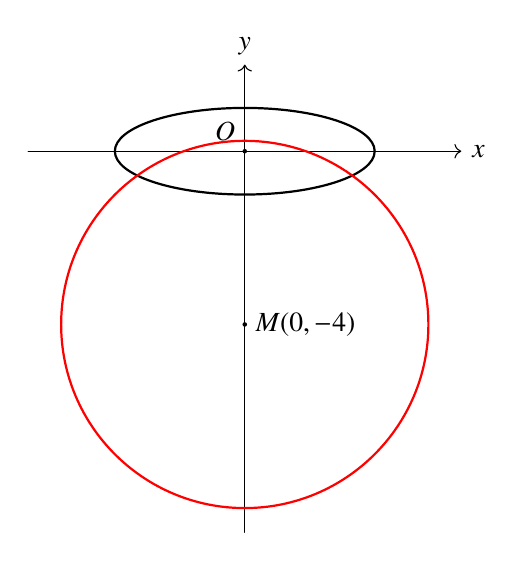
\begin{tikzpicture}[scale=0.55, line cap=round, line join=round]
				\draw[->] (-5,0)--(5,0) node[right]{$x$};
				\draw[->] (0,-8.8)--(0,2) node[above]{$y$};
				\draw[thick] (0,0) ellipse (3 and 1);
				\draw[thick, red] (0,-4) circle (4.24);
				\fill (0,-4) circle(1.5pt) node[right]{$M(0,-4)$};
				\fill (0,0) circle(1.5pt) node[above left]{$O$};
			\end{tikzpicture}
		\end{center}
		
		\item (17分)\\
		(1) 设函数$f(x)=5\cos x-\cos5x$，求$f(x)$在$\left[0,\dfrac{\pi}{4}\right]$的最大值；
		
		(2) 给定$\theta\in(0,\pi)$，设$a$为实数，证明：存在$y\in[a-\theta,a+\theta]$，使得$\cos y\le\cos\theta$；
		
		(3) 若存在$\varphi$使得对任意$x$，都有$5\cos x-\cos(5x+\varphi)\le b$，求$b$的最小值.
		
		\textbf{【答案】}(1) $3\sqrt3$；(3) $6$.
		
		\textbf{【详解】}(1) $f'(x)=-5\sin x+5\sin5x=10\cos3x\sin2x$.
		
		当$x\in\left[0,\dfrac{\pi}{6}\right)$时$f'(x)>0$，
		
		当$x\in\left(\dfrac{\pi}{6},\dfrac{\pi}{4}\right]$时$f'(x)<0$，
		
		故$f(x)$在$\left[0,\dfrac{\pi}{6}\right]$上增、在$\left[\dfrac{\pi}{6},\dfrac{\pi}{4}\right]$上减，
		
		最大值为$f\left(\dfrac{\pi}{6}\right)=5\cos\dfrac{\pi}{6}-\cos\dfrac{5\pi}{6}=\dfrac{5\sqrt3}{2}+\dfrac{\sqrt3}{2}=3\sqrt3$.
		
		(2) （反证法）由余弦性质，$\cos y>\cos\theta$的解为$2k\pi-\theta<y<2k\pi+\theta\ (k\in\mathbb{Z})$.
		
		若对任意$y\in[a-\theta,a+\theta]$都有$\cos y>\cos\theta$，
		
		则闭区间$[a-\theta,a+\theta]$必含于某个开区间$(2k\pi-\theta,2k\pi+\theta)$内.
		
		但前者长度为$2\theta$，后者长度也为$2\theta$，
		
		长度为$2\theta$的闭区间不可能含于长度为$2\theta$的开区间，矛盾.
		
		故存在$y\in[a-\theta,a+\theta]$，使得$\cos y\le\cos\theta$.
		
		(3) 记$g(x)=5\cos x-\cos(5x+\varphi)$.
		
		一方面，取$\varphi=\pi$，则$g(x)=5\cos x+\cos5x\le5+1=6$，且$x=0$时取等，
		
		即$b=6$可以取到；
		
		另一方面，若$b<6$，即对任意$x$有$5\cos x-\cos(5x+\varphi)\le b<6$，
		
		取$x=0,\ \dfrac{2\pi}{5},\ \dfrac{4\pi}{5}$分析：三个角$\dfrac{5x+\varphi}{1}$对应的单位圆上的点将单位圆三等分，
		
		不可能同时位于直线左侧，推出矛盾，
		
		故$b\ge6$.
		
		综上，$b$的最小值是$6$.
		
	\end{enumerate}
\end{document}